% !TeX program = xelatex
\documentclass[t, aspectratio=169, 11pt]{beamer}

\usepackage{fontspec}
\setmainfont{Times New Roman}
\setsansfont{Arial}
\setmonofont[Scale=0.9]{Courier New}
\usepackage{amsthm,amsmath,amssymb,mathtools}
\usepackage{bm}
\usepackage{array,booktabs,multirow,makecell}
\usepackage{colortbl}
\usepackage{tikz}
\usepackage[normalem]{ulem}
\usepackage{etoolbox}
\usetikzlibrary{positioning,calc,arrows.meta,backgrounds,shapes.geometric}

\makeatletter
\patchcmd{\beamer@sectionintoc}{\vskip1.5em}{\vskip0.55em}{}{}
\makeatother

% --- CẤU HÌNH LỀ ---
\def\slideContentLeftMargin{0.5cm}
\def\slideContentRightMargin{1cm}
\def\hustHeaderHeight{1cm}
\def\slideContentBotMargin{2.5cm}
\def\slideContentTopPadding{0.55cm}

\usepackage[red, 169]{beamerthemeHUST}

\graphicspath{{images/}{../reports/figures/}{./}}

\setbeamertemplate{footline}{\vspace{1.45cm}}
\setbeamertemplate{itemize item}{\textbullet}
\setbeamertemplate{itemize subitem}{\small\textbullet}
\setbeamertemplate{itemize subsubitem}{\small\textbullet}
\setbeamercolor{itemize item}{fg=black!80}
\setbeamercolor{itemize subitem}{fg=black!70}
\setbeamercolor{itemize subsubitem}{fg=black!70}

% Cỡ chữ body nhỏ lại để chứa nhiều ý mà KHÔNG tràn khỏi frame
\setbeamerfont{itemize/enumerate body}{size=\small}
\setbeamerfont{itemize/enumerate subbody}{size=\footnotesize}
\setbeamerfont{itemize/enumerate subsubbody}{size=\footnotesize}

% Siết khoảng cách dòng/đề mục trong itemize
\makeatletter
\def\@listi{\leftmargin\leftmargini \topsep 1pt \parsep 0pt \itemsep 3pt}
\let\@listI\@listi
\makeatother

\setlength{\leftmargini}{1.3em}
\setbeamertemplate{frametitle continuation}{}

\renewcommand{\titlePageTitleX}{-0.5cm}
\renewcommand{\titlePageTitleY}{-0.5cm}
\renewcommand{\hustTitleAlign}{\alignLeft}
\renewcommand{\hustSubtitleAlign}{\alignLeft}
\renewcommand{\hustAuthorAlign}{\alignLeft}
\renewcommand{\hustInstAlign}{\alignLeft}

% Macro tiện ích
\newcommand{\blk}[1]{\textbf{\color{hustprimary}#1}}
\newcommand{\readfig}[1]{\par\vspace{2pt}{\scriptsize\itshape\color{black!65}#1}}
% Nhãn cho các phần mở rộng
\newcommand{\mr}{{\footnotesize\color{black!55}[Mở rộng]}\ }

\title{Hệ hỗ trợ quyết định điều phối giao Pizza}
\subtitle{Từ dữ liệu đơn hàng đến dự đoán đơn trễ và quyết định điều phối}
\author{
  \textbf{Nhóm 29} \\
  \small
  Đoàn Danh Long (20237354) \quad Vũ Quang Vinh (20237408) \\
  Nguyễn Đăng Đức (20237312) \quad Nguyễn Tuấn Anh (20237293)
}
\institute{
  Đại học Bách khoa Hà Nội -- Khoa Toán Tin \\
  Giảng viên: TS. Lê Hải Hà \quad \quad Hướng dẫn TH: TS. Trịnh Đình Thăng
}
\date{Tháng 6 năm 2026}

\begin{document}

% =====================================================================
\husttitlepage

% =====================================================================
% Mục lục
% =====================================================================
\begin{frame}{Nội dung trình bày}
    \begin{columns}[T]
        \column{0.5\linewidth}
        \blk{Phần I — Bài toán \& dữ liệu}
        \begin{itemize}\small
            \item Bài toán \& quyết định cần hỗ trợ
            \item Dữ liệu \& chống rò rỉ thông tin
            \item Suy luận ngưỡng trễ, truy vết dữ liệu
        \end{itemize}
        \vspace{0.2cm}
        \blk{Phần II — Dự đoán đơn trễ}
        \begin{itemize}\small
            \item Yếu tố gây trễ (phân tích dữ liệu)
            \item Chọn đặc trưng \& so sánh mô hình
            \item Tinh chỉnh, ngưỡng \& độ ổn định
            \item Kết quả kiểm thử so với baseline
        \end{itemize}

        \column{0.5\linewidth}
        \blk{Phần III — Từ dự đoán đến quyết định}
        \begin{itemize}\small
            \item Điểm rủi ro \& bóc tách thành phần
            \item Hiệu chuẩn \& độ nhạy ngưỡng
            \item Hàng đợi ưu tiên \& hành động
            \item Xếp tài xế (bài toán phân công)
        \end{itemize}
        \vspace{0.2cm}
        \blk{Phần IV — Mở rộng \& trình bày}
        \begin{itemize}\small
            \item Phân tích nghiệp vụ mở rộng
            \item Bảng điều khiển \& bộ dữ liệu báo cáo
            \item Phản biện, giới hạn \& kết luận
        \end{itemize}
    \end{columns}
\end{frame}

% =====================================================================
% PHẦN I — BÀI TOÁN & DỮ LIỆU
% =====================================================================

\begin{frame}{1. Bài toán \& quyết định cần hỗ trợ}
    \begin{columns}[T]
        \column{0.5\linewidth}
        \blk{Bối cảnh}
        \begin{itemize}
            \item Giờ cao điểm nhiều đơn, tài xế \& bếp có hạn nên một số đơn bị trễ, khách phật ý.
            \item Quản lý cần biết \textbf{trước} đơn nào dễ trễ để lo liệu kịp.
        \end{itemize}
        \vspace{0.12cm}
        \blk{Hệ thống hỗ trợ ra sao?}
        \begin{itemize}
            \item \textbf{Đầu vào:} thông tin đơn ngay lúc tiếp nhận (trước khi giao).
            \item \textbf{Dự đoán:} ước lượng khả năng đơn bị trễ.
            \item \textbf{Đề xuất:} chấm điểm rủi ro, xếp mức ưu tiên, gợi ý hành động và xếp tài xế.
        \end{itemize}

        \column{0.48\linewidth}
        \centering
        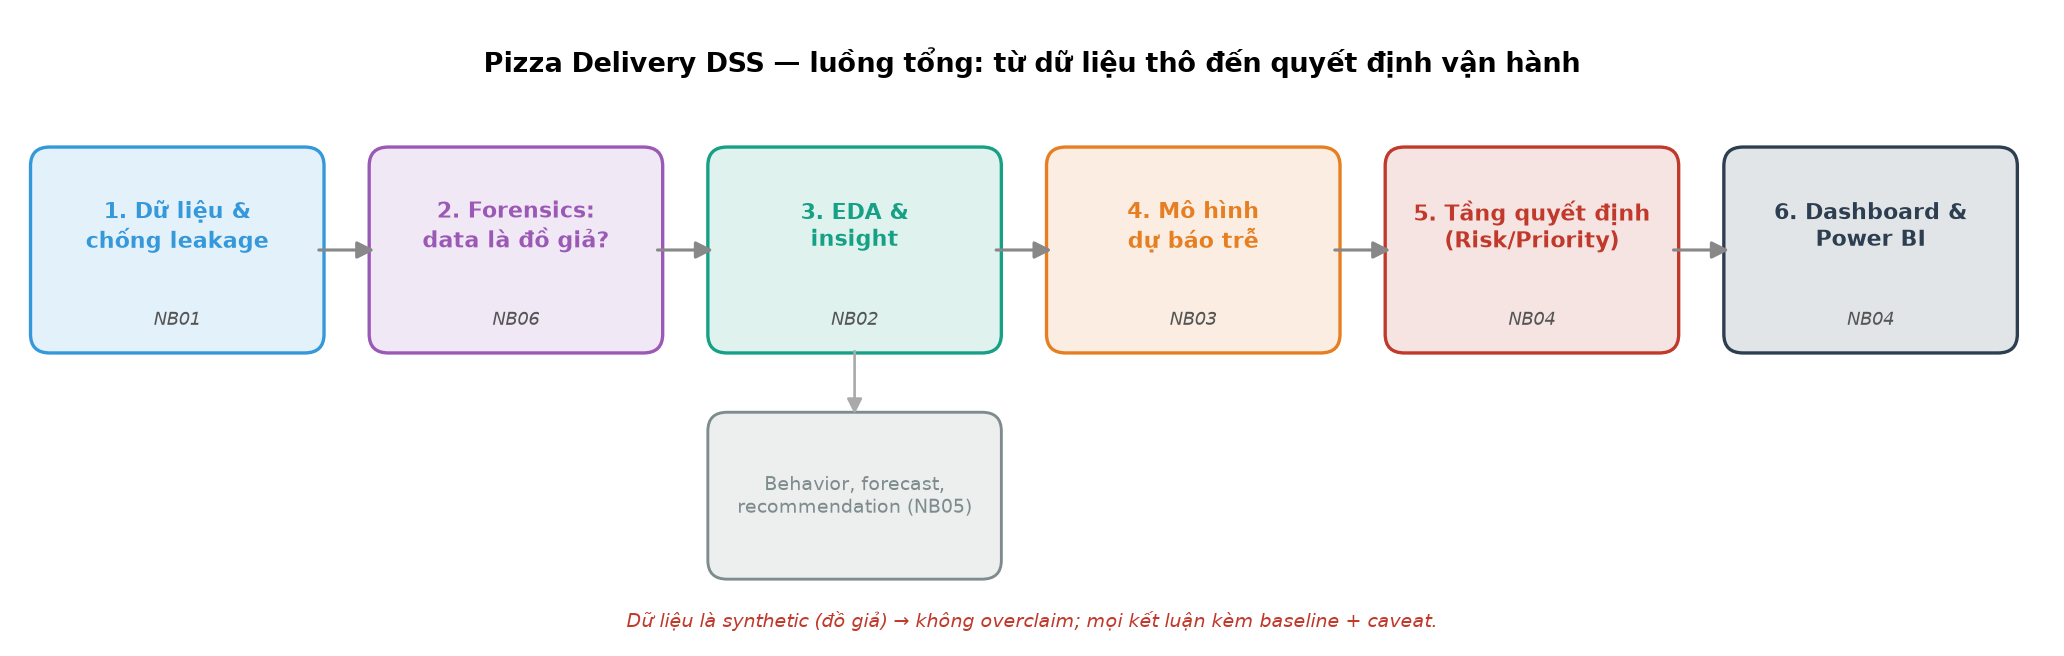
\includegraphics[width=\linewidth,height=0.62\textheight,keepaspectratio]{pipeline_overview.png}
        \readfig{Mạch xử lý xuyên suốt: từ dữ liệu đơn đến quyết định điều phối.}
    \end{columns}
\end{frame}

\begin{frame}{2. Dữ liệu \& chống rò rỉ thông tin}
    \begin{columns}[T]
        \column{0.52\linewidth}
        \blk{Bộ dữ liệu}
        \begin{itemize}
            \item Nguồn Kaggle: 1.004 đơn, 25 cột gốc.
            \item Mục tiêu cần dự đoán: nhãn đơn có trễ hay không.
        \end{itemize}
        \vspace{0.12cm}
        \blk{Nguyên tắc chống rò rỉ}
        \begin{itemize}
            \item Chỉ dùng thông tin \textbf{biết được lúc nhận đơn}.
            \item Loại bỏ các cột chỉ có \textit{sau khi giao xong}:
            \begin{itemize}\footnotesize
                \item thời gian giao, độ trễ thực tế
                \item hiệu suất giao, thời gian trung bình của cửa hàng
            \end{itemize}
        \end{itemize}

        \column{0.46\linewidth}
        \centering
        \blk{Vì sao quan trọng?}\par\vspace{4pt}
        \footnotesize
        Nhãn ``trễ'' được sinh \textbf{trực tiếp} từ thời gian giao. Đưa thời gian
        giao vào mô hình chẳng khác nào cho nó xem trước đáp án — đây là lỗi
        \emph{rò rỉ dữ liệu} kinh điển mà môn học luôn nhắc phải tránh.
    \end{columns}
\end{frame}

\begin{frame}{3. Suy luận ngưỡng trễ từ chính dữ liệu}
    \begin{columns}[T]
        \column{0.5\linewidth}
        \blk{Vấn đề}
        \begin{itemize}
            \item Dữ liệu không kèm cam kết thời gian giao, nên không biết bao nhiêu phút thì tính ``trễ''.
        \end{itemize}
        \vspace{0.12cm}
        \blk{Cách làm: dò ngưỡng}
        \begin{itemize}
            \item Thử mọi mốc thời gian rồi đối chiếu với nhãn gốc.
            \item Mọi đơn quá \textbf{30 phút} đều bị gắn ``trễ'' — khớp \textbf{tuyệt đối}, không sai lệch.
            \item Do thời gian giao chỉ rơi vào bội số của 5, mốc 30 và 35 phút cho kết quả như nhau.
        \end{itemize}
        \vspace{0.12cm}
        \blk{Kết luận} Ngưỡng trễ là \textbf{30 phút} — rút ra từ dữ liệu, không tự đặt.

        \column{0.48\linewidth}
        \centering
        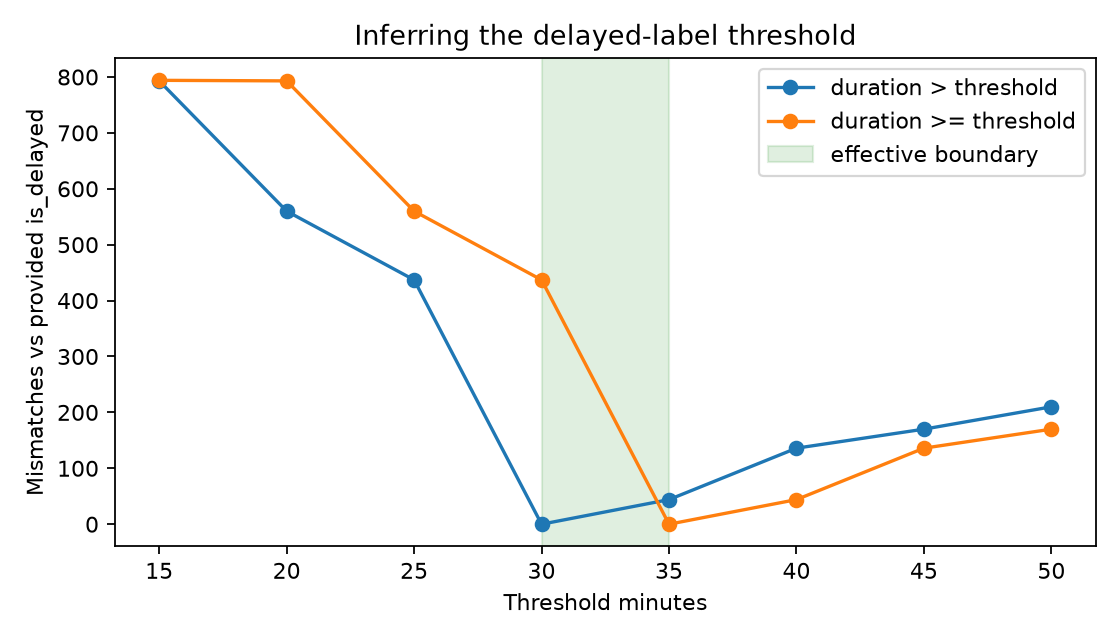
\includegraphics[width=\linewidth,height=0.58\textheight,keepaspectratio]{delay_threshold_inference.png}
        \readfig{Độ lệch chạm 0 ở vùng ngưỡng 30--35 phút.}
    \end{columns}
\end{frame}

\begin{frame}{4. Truy vết dữ liệu giả lập — vì sao cần?}
    \begin{columns}[T]
        \column{0.54\linewidth}
        \blk{Lý do}
        \begin{itemize}
            \item Bộ dữ liệu này thực ra do \textbf{máy sinh tự động}, không phải đơn hàng thật.
            \item Không vạch ra điều đó thì rất dễ \emph{thổi phồng}: tưởng mô hình giỏi và các phân tích là sự thật thị trường.
        \end{itemize}
        \vspace{0.12cm}
        \blk{Quan điểm của nhóm}
        \begin{itemize}
            \item \textbf{Không che giấu} điểm yếu dữ liệu — biến nó thành một phần phân tích có giá trị.
            \item Vẫn chạy \textbf{trọn vẹn quy trình} môn học để thể hiện năng lực, nhưng luôn kèm ghi chú trung thực.
        \end{itemize}

        \column{0.44\linewidth}
        \centering
        \footnotesize
        \blk{Thông điệp cốt lõi}\par\vspace{4pt}
        Điểm mô hình cao \textbf{không} đồng nghĩa đoán giỏi ngoài đời. Điểm cao
        đến từ việc dữ liệu được sinh theo công thức gần như cố định — và chính
        phần truy vết này chứng minh điều đó.
    \end{columns}
\end{frame}

\begin{frame}{5. Truy vết — bằng chứng dữ liệu tất định}
    \begin{columns}[T]
        \column{0.5\linewidth}
        \blk{Bảy công thức cố định}
        \begin{itemize}
            \item Dựng lại được \textbf{7 công thức} khớp tuyệt đối giữa các biến (sai số gần như bằng 0).
            \item Ví dụ: thời gian ước tính $= 2{,}4 \times$ quãng đường (đúng từng dòng).
            \item Độ phức tạp đơn $=$ số topping $\times$ điểm cỡ bánh.
        \end{itemize}
        \vspace{0.12cm}
        \blk{Hệ quả cho mô hình}
        \begin{itemize}
            \item Các biến này \textbf{trùng thông tin} nhau.
            \item Vì vậy bị loại khỏi bộ đặc trưng rút gọn (xem Phần II).
        \end{itemize}

        \column{0.48\linewidth}
        \centering
        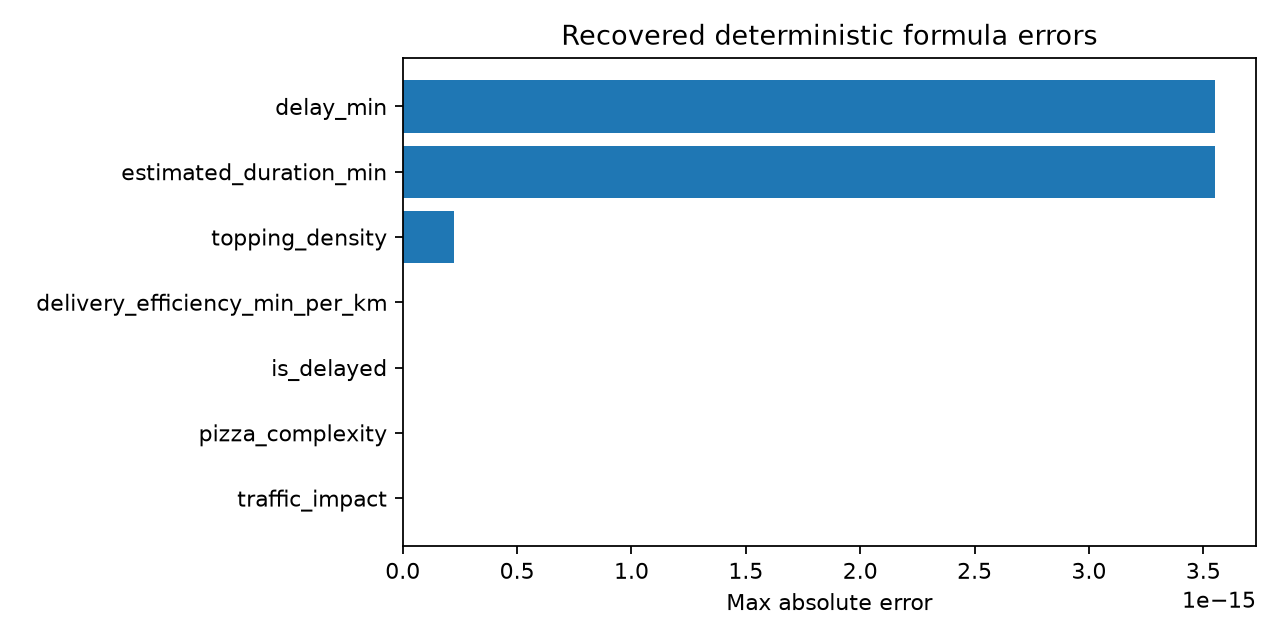
\includegraphics[width=\linewidth,height=0.6\textheight,keepaspectratio]{generator_deterministic_formula_errors.png}
        \readfig{Sai số dựng lại công thức cỡ $10^{-15}$ — tức là cố định.}
    \end{columns}
\end{frame}

% =====================================================================
% PHẦN II — DỰ ĐOÁN ĐƠN TRỄ
% =====================================================================

\begin{frame}{6. Yếu tố gây trễ: phân phối nhãn \& cách đánh giá}
    \begin{columns}[T]
        \column{0.5\linewidth}
        \blk{Lệch lớp}
        \begin{itemize}
            \item 1.004 đơn nhưng chỉ 210 đơn trễ ($\sim 20{,}92\%$) — số đơn trễ ít hơn hẳn.
        \end{itemize}
        \vspace{0.12cm}
        \blk{Hệ quả: không nhìn mỗi độ chính xác}
        \begin{itemize}
            \item Cứ đoán ``mọi đơn đều đúng giờ'' đã đạt độ chính xác 79\%, nhưng bắt được \textbf{0 đơn trễ} — vô dụng.
            \item Phải xét thêm F2, MCC, độ chính xác cân bằng.
            \item Lấy \textbf{F2} làm thước đo chính: phạt nặng việc \emph{bỏ sót} đơn trễ.
        \end{itemize}

        \column{0.48\linewidth}
        \centering
        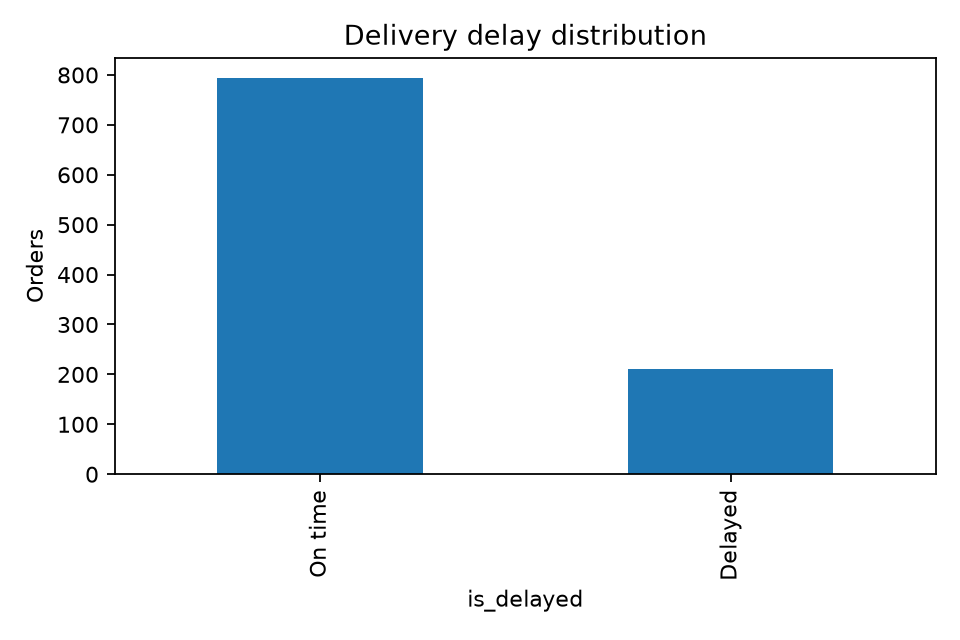
\includegraphics[width=\linewidth,height=0.6\textheight,keepaspectratio]{delay_distribution.png}
        \readfig{Cột ``đúng giờ'' cao gấp khoảng 4 lần cột ``trễ''.}
    \end{columns}
\end{frame}

\begin{frame}{7. Yếu tố gây trễ: giao thông đứng đầu}
    \begin{columns}[T]
        \column{0.5\linewidth}
        \blk{Mức độ giao thông}
        \begin{itemize}
            \item Khi đường đông (mức cao), tỷ lệ trễ tăng vọt.
            \item Mức vừa và thấp thì tỷ lệ trễ thấp hơn hẳn.
            \item Đây là yếu tố vận hành quan trọng nhất, cần theo dõi sát.
        \end{itemize}
        \vspace{0.12cm}
        \blk{Dùng vào đâu?}
        \begin{itemize}
            \item Giao thông là một thành phần của điểm rủi ro (Phần III).
            \item Lưu ý: đây là tương quan, \textbf{không} khẳng định nhân quả.
        \end{itemize}

        \column{0.48\linewidth}
        \centering
        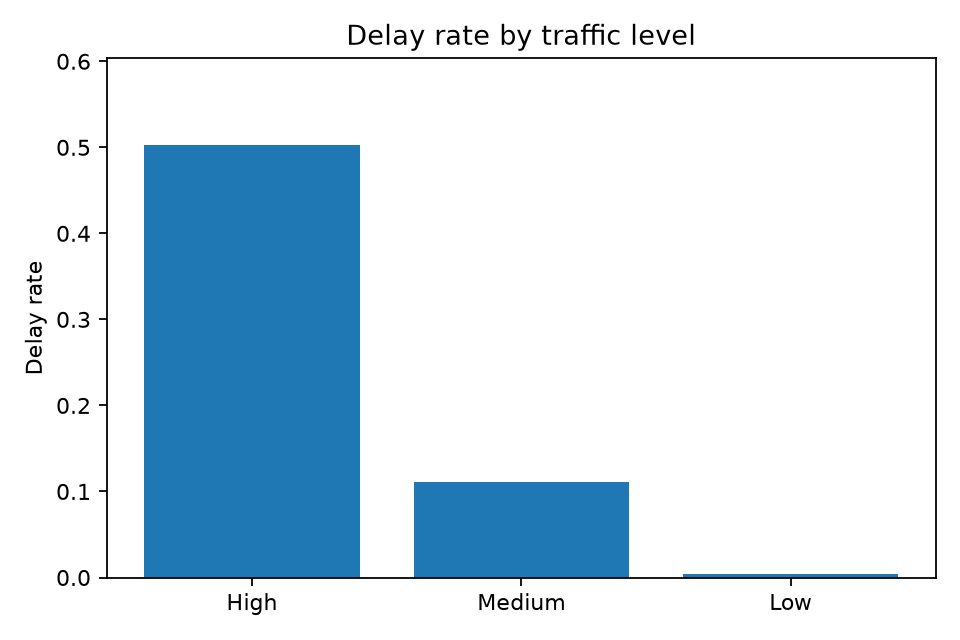
\includegraphics[width=\linewidth,height=0.6\textheight,keepaspectratio]{delay_rate_by_traffic.png}
        \readfig{Tỷ lệ trễ theo mức giao thông: cao $\gg$ vừa $>$ thấp.}
    \end{columns}
\end{frame}

\begin{frame}{8. Yếu tố gây trễ: quãng đường \& độ phức tạp}
    \begin{columns}[T]
        \column{0.5\linewidth}
        \blk{Quãng đường}
        \begin{itemize}
            \item Đơn càng xa, thời gian di chuyển càng tăng (gần như tuyến tính).
            \item Xa \textbf{cộng thêm} đường đông thì gần như chắc chắn trễ.
        \end{itemize}
        \vspace{0.12cm}
        \blk{Độ phức tạp đơn}
        \begin{itemize}
            \item Nhiều topping \& bánh cỡ lớn làm tăng thời gian chuẩn bị ở bếp.
            \item Mức đóng góp vào rủi ro \textbf{nhỏ hơn} giao thông và quãng đường.
        \end{itemize}

        \column{0.48\linewidth}
        \centering
        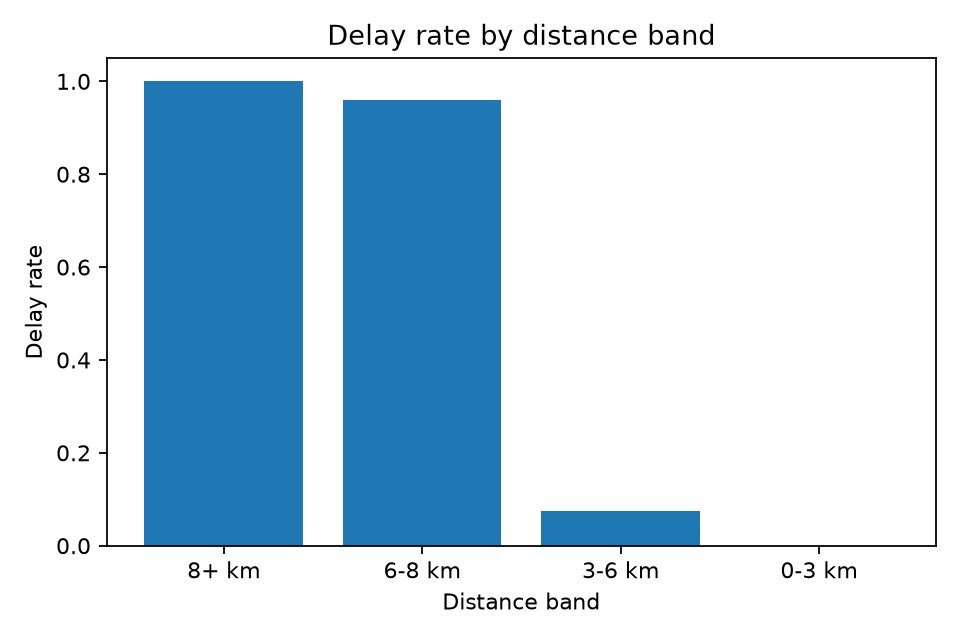
\includegraphics[width=\linewidth,height=0.6\textheight,keepaspectratio]{delay_rate_by_distance_band.png}
        \readfig{Tỷ lệ trễ tăng dần theo dải quãng đường.}
    \end{columns}
\end{frame}

\begin{frame}{9. Chọn đặc trưng: rút gọn hay đầy đủ?}
    \begin{columns}[T]
        \column{0.5\linewidth}
        \blk{Hai bộ đặc trưng}
        \begin{itemize}
            \item \textbf{Đầy đủ (17):} mọi biến biết được trước khi giao.
            \item \textbf{Rút gọn (12):} bỏ các biến cố định/trùng thông tin (từ truy vết) và biến gây nhiễu.
        \end{itemize}
        \vspace{0.12cm}
        \blk{Vì sao ưu tiên bộ rút gọn?}
        \begin{itemize}
            \item Tránh các biến trùng nhau, mô hình gọn và ít học tủ.
            \item Kết quả so sánh ở trang sau.
        \end{itemize}

        \column{0.48\linewidth}
        \centering
        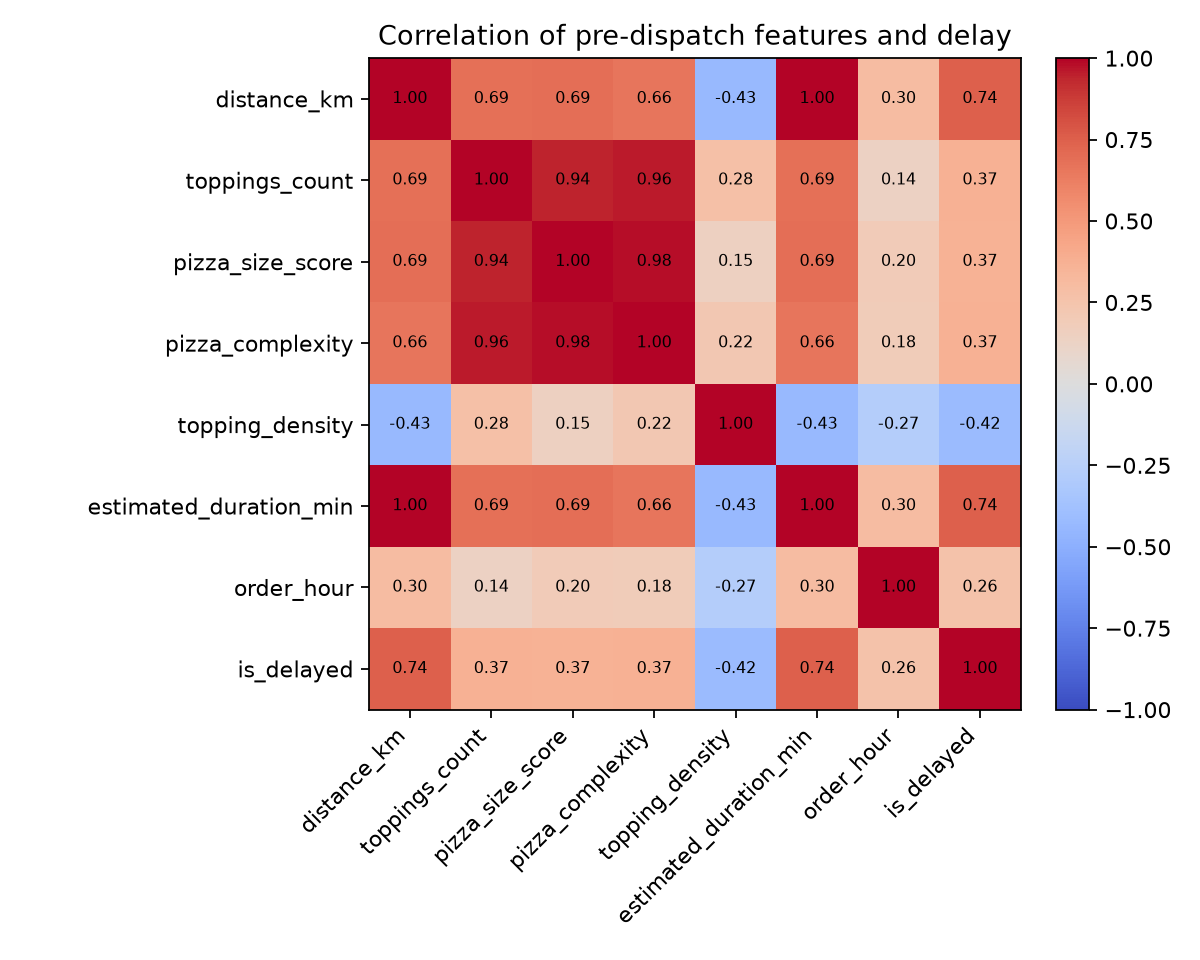
\includegraphics[width=\linewidth,height=0.6\textheight,keepaspectratio]{correlation_heatmap.png}
        \readfig{Nhiều ô đỏ đậm = các biến tương quan mạnh, trùng thông tin.}
    \end{columns}
\end{frame}

\begin{frame}{10. Bộ rút gọn thắng bộ đầy đủ}
    \begin{columns}[T]
        \column{0.46\linewidth}
        \begin{table}
            \centering\small
            \renewcommand{\arraystretch}{1.2}
            \begin{tabular}{lrr}
            \toprule
            \textbf{Bộ đặc trưng} & \textbf{F2} & \textbf{MCC}\\
            \midrule
            Rút gọn (12) & \textbf{0.9434} & \textbf{0.9117}\\
            Đầy đủ (17)  & 0.9286 & 0.9097\\
            \bottomrule
            \end{tabular}
        \end{table}

        \column{0.52\linewidth}
        \blk{Đọc bảng}
        \begin{itemize}
            \item Bộ rút gọn \textbf{cao hơn} ở cả F2 lẫn MCC dù dùng ít biến hơn.
            \item Khẳng định: bỏ biến trùng thông tin \textbf{không làm giảm} sức dự đoán, mà còn giúp mô hình ổn định, dễ giải thích.
            \item Vì vậy khoá lại \textbf{bộ rút gọn 12 biến} cho các bước sau.
        \end{itemize}
    \end{columns}
\end{frame}

\begin{frame}{11. So sánh sáu mô hình dự đoán}
    \begin{columns}[T]
        \column{0.5\linewidth}
        \blk{Xếp hạng theo F2}
        \begin{itemize}
            \item \textbf{Hồi quy Logistic:} F2 = 0.9434, MCC = 0.9117 — \textbf{tốt nhất} và dễ giải thích.
            \item SVM (0.9048), Cây quyết định (0.8962): khá nhưng phức tạp hơn.
            \item Rừng ngẫu nhiên (0.8780): học tủ mạnh.
            \item k láng giềng (0.7538): yếu hơn rõ rệt.
        \end{itemize}
        \vspace{0.1cm}
        \blk{Chốt} Chọn \textbf{Hồi quy Logistic} theo F2.

        \column{0.48\linewidth}
        \centering
        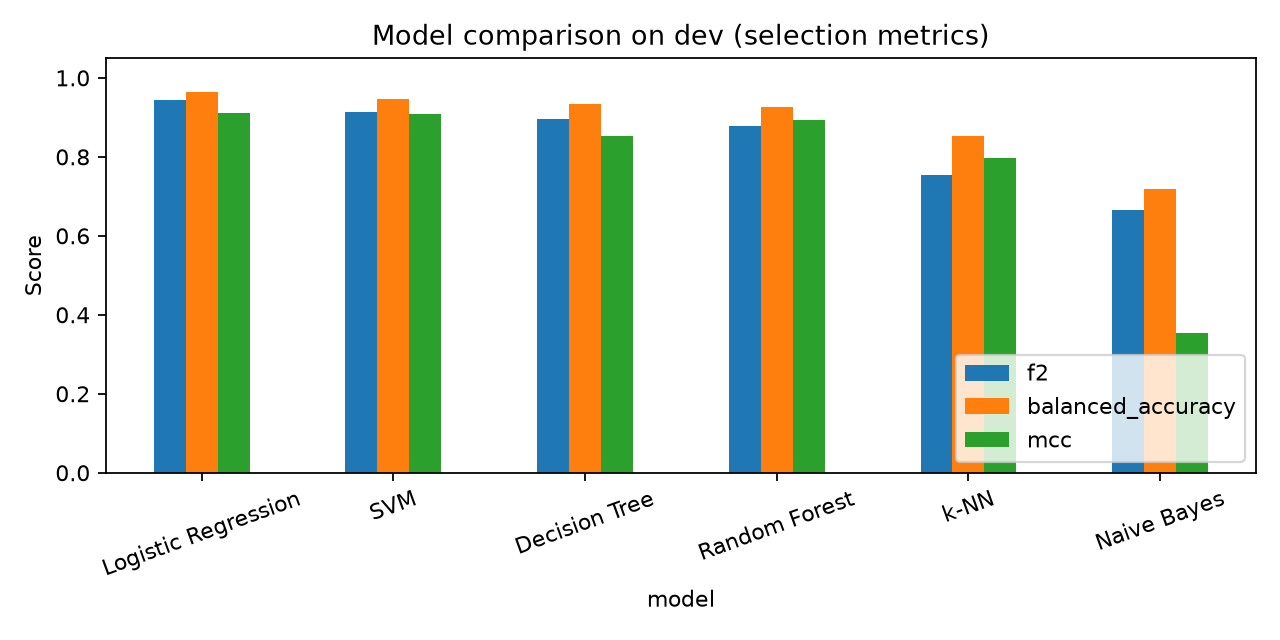
\includegraphics[width=\linewidth,height=0.6\textheight,keepaspectratio]{model_comparison.png}
        \readfig{Cụm cột của Hồi quy Logistic cao \& đều nhất.}
    \end{columns}
\end{frame}

\begin{frame}{12. Vì sao không chọn Naive Bayes?}
    \begin{columns}[T]
        \column{0.54\linewidth}
        \blk{Điểm số thấp hẳn}
        \begin{itemize}
            \item Naive Bayes: F2 chỉ \textbf{0.6642}, MCC \textbf{0.3544} — thấp nhất trong sáu mô hình.
        \end{itemize}
        \vspace{0.15cm}
        \blk{Nguyên nhân}
        \begin{itemize}
            \item Naive Bayes giả định các biến \textbf{độc lập} với nhau.
            \item Ở đây quãng đường, địa điểm, giao thông \textbf{liên kết chặt} (đã thấy ở phần phân tích) nên giả định bị vi phạm nặng.
            \item Vì thế nhóm đã \emph{thử} nhưng \textbf{không chọn} — không phải bỏ qua.
        \end{itemize}

        \column{0.44\linewidth}
        \centering
        \footnotesize
        \blk{Bài học}\par\vspace{4pt}
        Chọn mô hình phải xét xem \textbf{giả định} của nó có hợp với dữ liệu hay
        không, chứ không chỉ nhìn điểm số.
    \end{columns}
\end{frame}

\begin{frame}{13. Tinh chỉnh siêu tham số}
    \begin{columns}[T]
        \column{0.54\linewidth}
        \blk{Quy tắc: chọn xong mới tinh chỉnh}
        \begin{itemize}
            \item Chỉ tinh chỉnh \textbf{sau khi} Hồi quy Logistic đã thắng vòng so sánh.
            \item Dò tham số trên tập huấn luyện bằng kiểm định chéo 5 phần, tối ưu theo F2.
        \end{itemize}
        \vspace{0.15cm}
        \blk{Kết quả \& quyết định}
        \begin{itemize}
            \item Bản tinh chỉnh lại cho F2 \textbf{thấp hơn} bản gốc trên tập kiểm định.
            \item Vì vậy \textbf{giữ cấu hình gốc} — minh bạch, không ép theo kiểm định chéo khi tập kiểm định nói ngược.
        \end{itemize}

        \column{0.44\linewidth}
        \centering
        \footnotesize
        \blk{Thông điệp}\par\vspace{4pt}
        Tinh chỉnh không phải lúc nào cũng tốt hơn. Nhóm báo cáo \textbf{trung
        thực} rằng bản gốc tốt hơn và giữ nó.
    \end{columns}
\end{frame}

\begin{frame}{14. Quét ngưỡng quyết định}
    \begin{columns}[T]
        \column{0.5\linewidth}
        \blk{Quét ngưỡng trên tập kiểm định}
        \begin{itemize}
            \item F2 ưu tiên bắt đúng đơn trễ: chấp nhận báo nhầm nhiều hơn để \textbf{không bỏ sót}.
            \item Ngưỡng tối ưu trên tập kiểm định cho tỷ lệ bắt đơn trễ đạt 100\%.
        \end{itemize}
        \vspace{0.12cm}
        \blk{Vì sao vẫn giữ ngưỡng 0.5?}
        \begin{itemize}
            \item Áp ngưỡng đó sang tập kiểm thử thì báo nhầm tăng mạnh, F2 lại giảm.
            \item Nên báo cáo chính giữ ngưỡng \textbf{0.5} cho ổn định.
        \end{itemize}

        \column{0.48\linewidth}
        \centering
        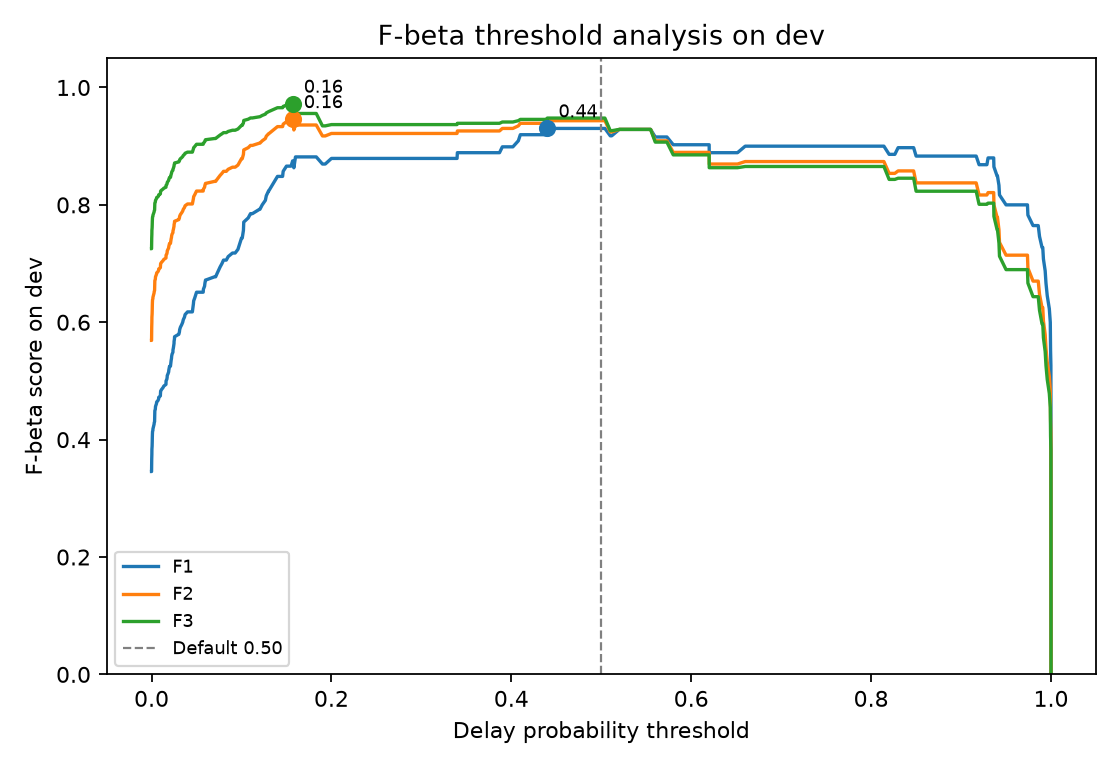
\includegraphics[width=\linewidth,height=0.6\textheight,keepaspectratio]{fbeta_threshold_curve.png}
        \readfig{Đường F2 phẳng ở vùng ngưỡng thấp — dễ học tủ theo tập kiểm định.}
    \end{columns}
\end{frame}

\begin{frame}{15. Kiểm thử độ ổn định (100 lần chia tập)}
    \begin{columns}[T]
        \column{0.5\linewidth}
        \blk{Mục tiêu}
        \begin{itemize}
            \item Trả lời câu hỏi: điểm cao có phải do \textbf{may mắn} một lần chia tập?
        \end{itemize}
        \vspace{0.12cm}
        \blk{Cách làm \& kết quả}
        \begin{itemize}
            \item Chia lại ngẫu nhiên \textbf{100 lần} trên dữ liệu huấn luyện (\textbf{không} đụng tập kiểm thử).
            \item F2 trung bình \textbf{0.9419}; dao động trong khoảng hẹp.
            \item Dao động nhỏ cho thấy mô hình \textbf{ổn định}, không ăn may.
        \end{itemize}

        \column{0.48\linewidth}
        \centering
        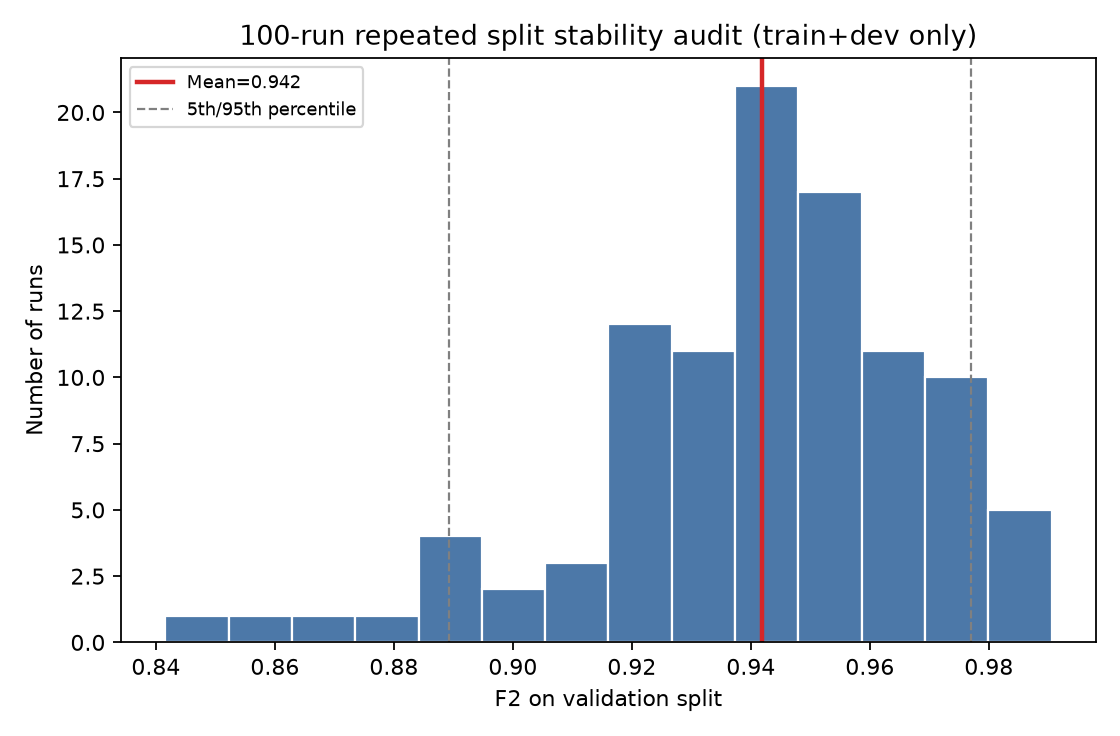
\includegraphics[width=\linewidth,height=0.6\textheight,keepaspectratio]{model_stability_f2_distribution.png}
        \readfig{Phân phối F2 qua 100 lần chia tập, tụm quanh 0.94.}
    \end{columns}
\end{frame}

\begin{frame}{16. Kết quả kiểm thử so với baseline}
    \begin{columns}[T]
        \column{0.45\linewidth}
        \blk{Hồi quy Logistic (kiểm thử)}
        \begin{table}
            \centering\small
            \renewcommand{\arraystretch}{1.1}
            \begin{tabular}{lr}
            \toprule
            \textbf{Thước đo} & \textbf{Giá trị}\\
            \midrule
            Độ chính xác & 0.9602\\
            Chính xác cân bằng & 0.9661\\
            Precision & 0.8542\\
            \textbf{Recall} & \textbf{0.9762}\\
            \textbf{F2} & \textbf{0.9491}\\
            MCC & 0.8889\\
            ROC-AUC & 0.9961\\
            \bottomrule
            \end{tabular}
        \end{table}

        \column{0.52\linewidth}
        \blk{So với hai baseline}
        \begin{itemize}
            \item ``Luôn đúng giờ'': độ chính xác 79,1\% nhưng F2 = 0, MCC = 0.
            \item ``Luôn trễ'': bắt hết đơn trễ nhưng độ chính xác chỉ 20,9\%, F2 = 0.569.
            \item Mô hình \textbf{vượt trội} cả hai ở các thước đo cân bằng; chỉ bỏ sót \textbf{1/42} đơn trễ.
        \end{itemize}
        \readfig{Nhắc lại: điểm cao một phần do dữ liệu gần như cố định.}
    \end{columns}
\end{frame}

% =====================================================================
% PHẦN III — TỪ DỰ ĐOÁN ĐẾN QUYẾT ĐỊNH
% =====================================================================

\begin{frame}{17. Điểm rủi ro: công thức tính (0--100)}
    \blk{Ý tưởng} Người điều phối không thể quyết chỉ bằng một con số xác suất khó
    hiểu. Ta kết hợp dự đoán của mô hình với \textbf{áp lực vận hành} thực tế thành
    một điểm rủi ro rõ ràng.
    \vspace{0.25cm}
    \begin{equation*}
    \begin{aligned}
        \text{Rủi ro} =\ & 0.55\,S_{\text{mô hình}} + 0.15\,S_{\text{giao thông}} + 0.12\,S_{\text{quãng đường}} \\
             &+\, 0.08\,S_{\text{cao điểm}} + 0.06\,S_{\text{phức tạp}} + 0.04\,S_{\text{cuối tuần}}
    \end{aligned}
    \end{equation*}
    \vspace{0.1cm}
    \begin{itemize}
        \item Mỗi thành phần được đưa về \textbf{thang 0--100} rồi mới nhân trọng số.
        \item Dự đoán của mô hình chiếm \textbf{55\%} (bằng chứng chính); 45\% còn lại là áp lực vận hành minh bạch.
        \item Đây là \textbf{chính sách do nhóm đặt}, không phải con số tối ưu thống kê.
    \end{itemize}
\end{frame}

\begin{frame}{18. Điểm rủi ro: bóc tách thành phần}
    \begin{columns}[T]
        \column{0.5\linewidth}
        \blk{Vì sao phải bóc tách?}
        \begin{itemize}
            \item Người điều phối thấy rõ \textbf{vì sao} một đơn bị chấm rủi ro cao, chứ không chỉ thấy con số cuối.
            \item Tăng độ tin và dễ điều chỉnh chính sách.
        \end{itemize}
        \vspace{0.12cm}
        \blk{Đọc biểu đồ}
        \begin{itemize}
            \item Phần dự đoán của mô hình đóng góp lớn nhất (đúng trọng số 0.55).
            \item Các áp lực vận hành bổ sung phần còn lại.
        \end{itemize}

        \column{0.48\linewidth}
        \centering
        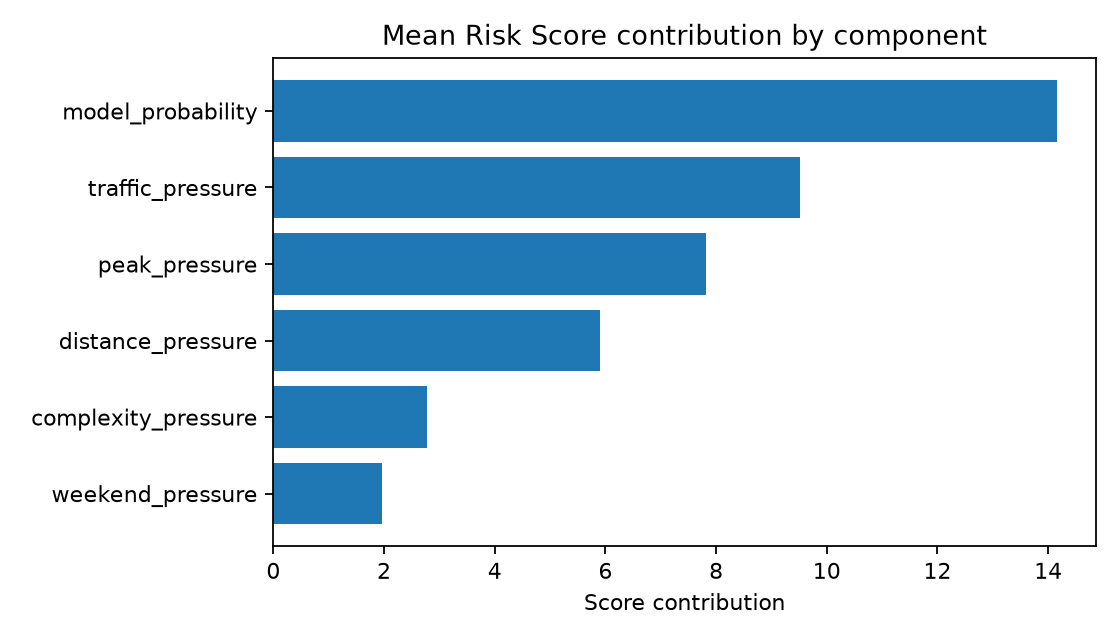
\includegraphics[width=\linewidth,height=0.6\textheight,keepaspectratio]{risk_component_breakdown.png}
        \readfig{Mức đóng góp trung bình của từng thành phần vào điểm rủi ro.}
    \end{columns}
\end{frame}

\begin{frame}{19. Hiệu chuẩn điểm rủi ro}
    \begin{columns}[T]
        \column{0.5\linewidth}
        \blk{Điểm rủi ro có ``đúng'' không?}
        \begin{itemize}
            \item Hiệu chuẩn = kiểm tra điểm rủi ro có khớp tỷ lệ trễ thực tế.
        \end{itemize}
        \vspace{0.12cm}
        \blk{Tỷ lệ trễ tăng dần theo nhóm}
        \begin{itemize}
            \item Nhóm thấp: trễ 0,0\%.
            \item Nhóm vừa: trễ 7,3\%.
            \item Nhóm cao: trễ tới \textbf{88,6\%}.
            \item Điểm càng cao, trễ càng nhiều — đúng kỳ vọng.
        \end{itemize}

        \column{0.48\linewidth}
        \centering
        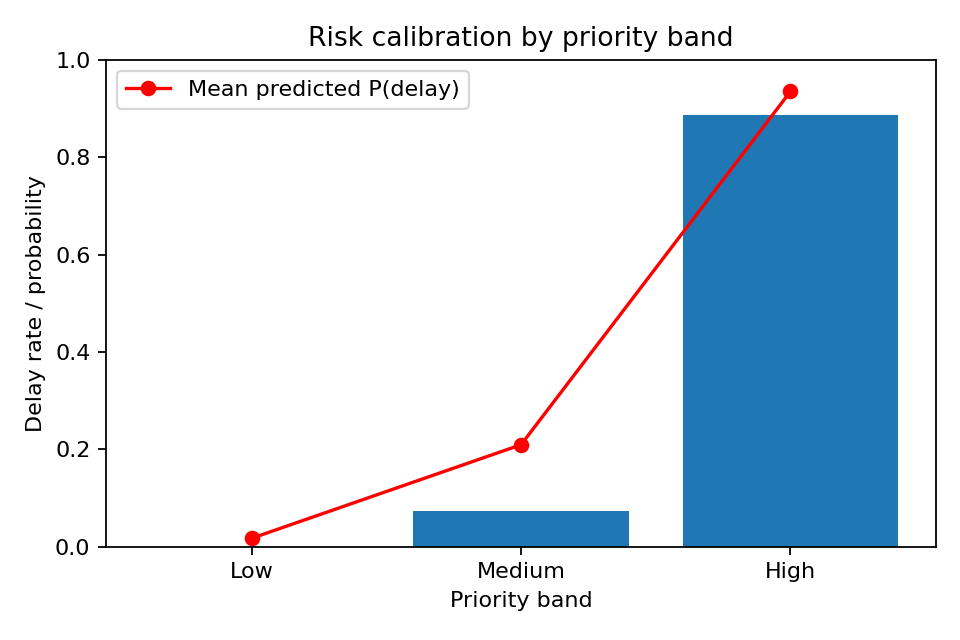
\includegraphics[width=\linewidth,height=0.6\textheight,keepaspectratio]{risk_calibration.png}
        \readfig{Đường tỷ lệ trễ thực tế đi lên đều theo nhóm.}
    \end{columns}
\end{frame}

\begin{frame}{20. Độ nhạy của ngưỡng ưu tiên}
    \begin{columns}[T]
        \column{0.5\linewidth}
        \blk{Ngưỡng phân nhóm}
        \begin{itemize}
            \item Thấp ($<35$) — Vừa ($35$--$65$) — Cao ($>65$).
        \end{itemize}
        \vspace{0.12cm}
        \blk{Đổi ngưỡng thì sao?}
        \begin{itemize}
            \item Nhóm cao hiện bắt được \textbf{92,9\%} tổng số đơn trễ.
            \item Hạ ngưỡng thì bắt được nhiều đơn hơn nhưng tốn nhân lực can thiệp.
            \item Ngưỡng là \textbf{nút điều chỉnh vận hành} để cân tải, không cố định cứng.
        \end{itemize}

        \column{0.48\linewidth}
        \centering
        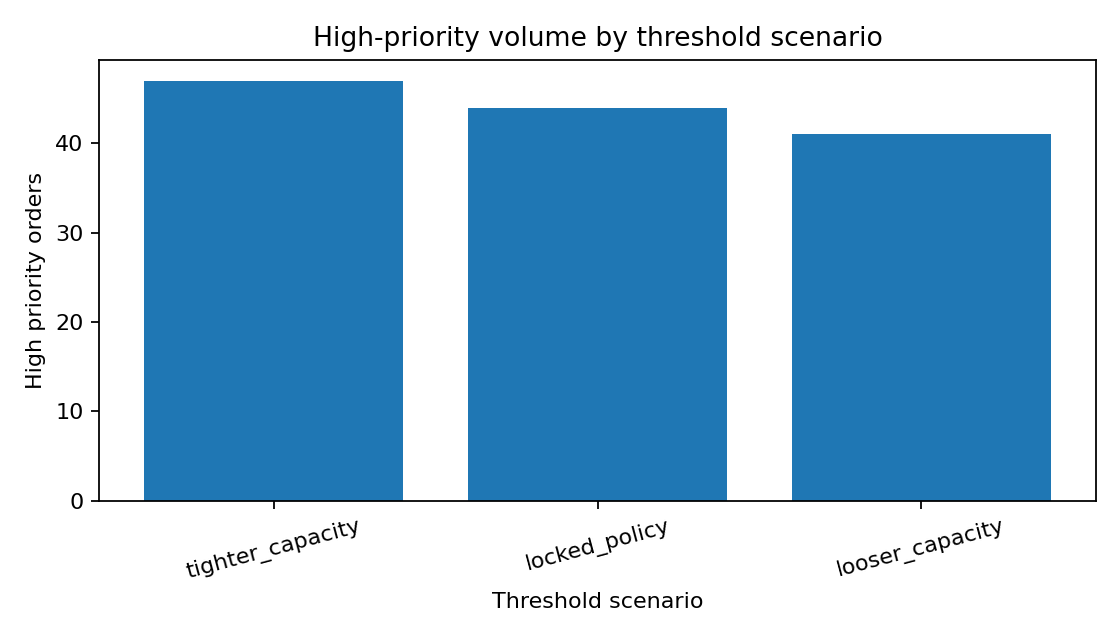
\includegraphics[width=\linewidth,height=0.6\textheight,keepaspectratio]{priority_threshold_sensitivity.png}
        \readfig{Số đơn nhóm cao \& số đơn trễ bắt được đổi theo ngưỡng.}
    \end{columns}
\end{frame}

\begin{frame}{21. Hàng đợi ưu tiên \& hành động}
    \begin{center}\small Điểm rủi ro được dịch thành hành động cụ thể cho người điều phối:\end{center}
    \vspace{-2pt}
    \begin{table}
        \centering\footnotesize
        \renewcommand{\arraystretch}{1.25}
        \begin{tabular}{p{1.9cm}p{2.6cm}p{8.3cm}}
        \toprule
        \textbf{Rủi ro} & \textbf{Mức ưu tiên} & \textbf{Hành động khuyến nghị}\\
        \midrule
        $> 65$ & \color{red}\textbf{Cao} & Xếp tài xế ưu tiên, đẩy lên đầu hàng đợi bếp, chuẩn bị tài xế dự phòng, sẵn sàng báo trễ cho khách.\\
        $35\text{--}65$ & \color{orange}\textbf{Vừa} & Theo dõi lộ trình \& tình hình giao thông; cập nhật giờ giao dự kiến nếu có biến động.\\
        $< 35$ & \color{green!60!black}\textbf{Thấp} & Xử lý theo quy trình thường, không cần can thiệp đặc biệt.\\
        \bottomrule
        \end{tabular}
    \end{table}
    \begin{center}\itshape\small
        Hàng đợi tự xếp đơn rủi ro cao lên đầu để điều phối xử lý ngay.
    \end{center}
\end{frame}

\begin{frame}{22. Xếp tài xế: bài toán phân công}
    \begin{columns}[T]
        \column{0.5\linewidth}
        \blk{Mô hình hoá}
        \begin{itemize}
            \item Lấy các đơn rủi ro cao từ hàng đợi (dữ liệu thật).
            \item Giả lập một đội tài xế: sức chở, vị trí xuất phát.
            \item Lập bảng chi phí: phạt khi đơn trễ không kịp giao, thưởng khi đi cùng tuyến.
            \item Giải tối ưu toàn cục bằng thuật toán phân công Hungary.
        \end{itemize}
        \vspace{0.1cm}
        \blk{Kết quả} Xếp \textbf{12 đơn} rủi ro cao cho \textbf{6 tài xế}, chi phí trung bình thấp nhất \textbf{32,84} — minh hoạ tầng đề xuất hành động.

        \column{0.48\linewidth}
        \centering
        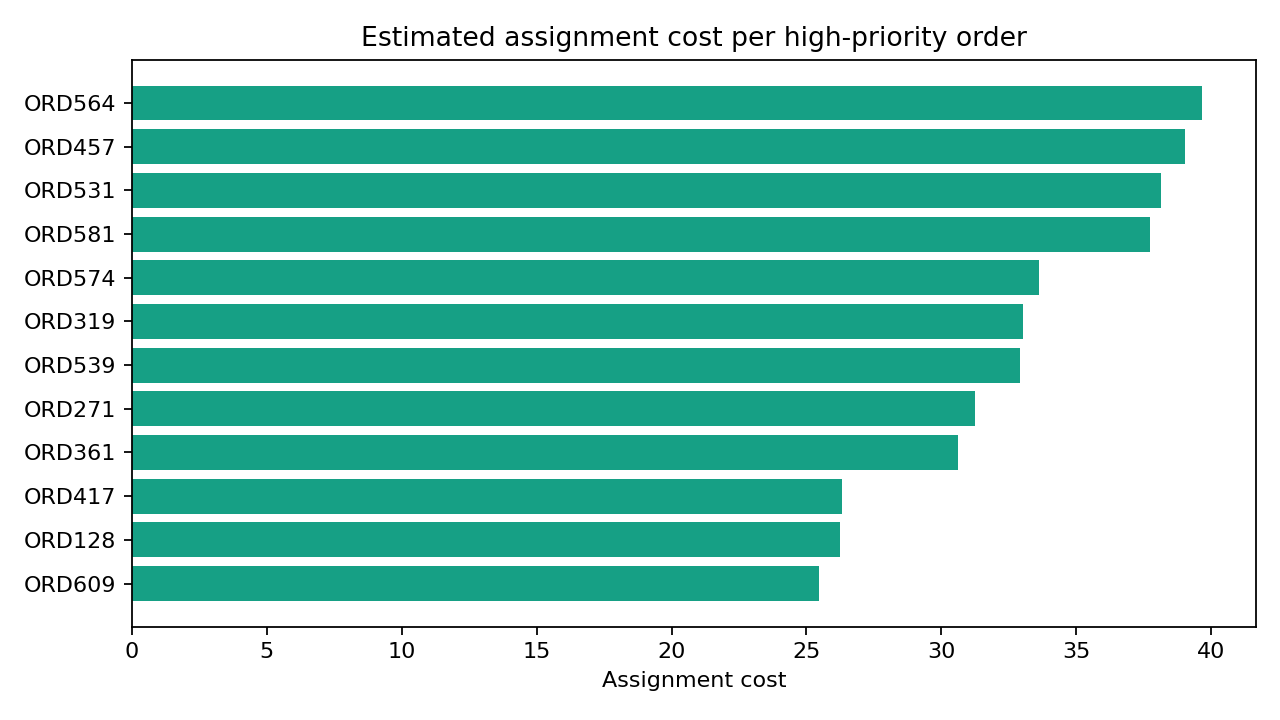
\includegraphics[width=\linewidth,height=0.6\textheight,keepaspectratio]{transport_assignment_cost.png}
        \readfig{Chi phí xếp theo từng cặp đơn--tài xế.}
    \end{columns}
\end{frame}

% =====================================================================
% PHẦN IV — MỞ RỘNG & TRÌNH BÀY
% =====================================================================

\begin{frame}{23. \mr Hành vi khách hàng}
    \begin{columns}[T]
        \column{0.5\linewidth}
        \blk{Cỡ bánh \& loại bánh}
        \begin{itemize}
            \item \textbf{Cỡ bánh:} cỡ vừa được đặt nhiều nhất (42,7\%), nhưng cỡ lớn và rất lớn lại trễ nhiều nhất.
            \item \textbf{Loại bánh:} mặn và chay chiếm đa số.
            \item \textbf{Topping:} chủ yếu 2--5 topping mỗi đơn.
        \end{itemize}
        \vspace{0.12cm}
        \blk{Lưu ý} Đây là dữ liệu giả lập — chỉ minh hoạ cách phân tích hành vi,
        \textbf{không} kết luận thị hiếu thật.

        \column{0.48\linewidth}
        \centering
        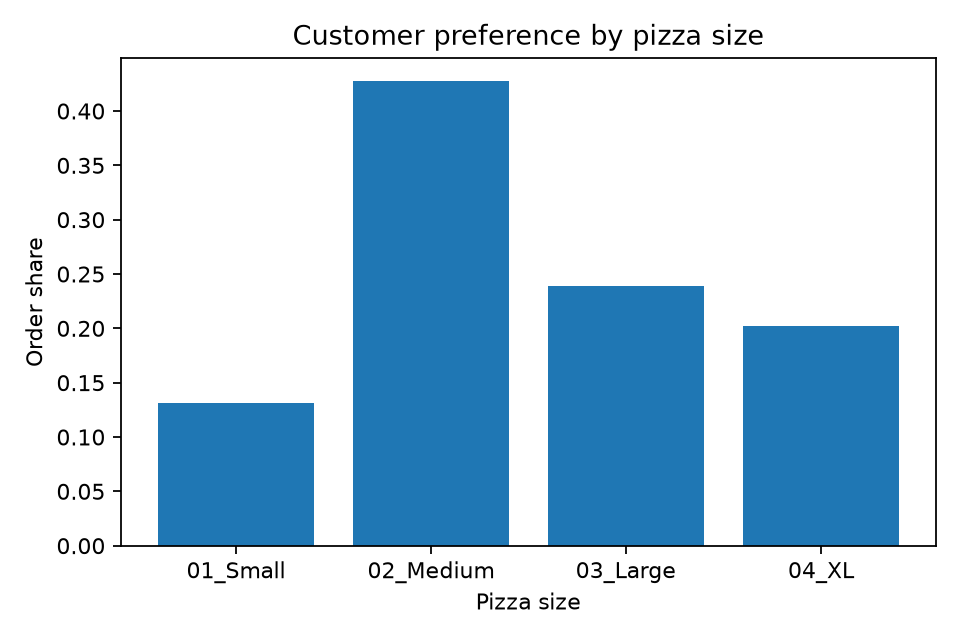
\includegraphics[width=\linewidth,height=0.6\textheight,keepaspectratio]{size_preference.png}
        \readfig{Tỷ trọng đặt hàng theo cỡ bánh.}
    \end{columns}
\end{frame}

\begin{frame}{24. \mr Dự báo nhu cầu theo tháng}
    \begin{columns}[T]
        \column{0.5\linewidth}
        \blk{Cách làm}
        \begin{itemize}
            \item Lấy nhu cầu cùng kỳ năm trước làm dự báo cho tháng tương ứng.
        \end{itemize}
        \vspace{0.12cm}
        \blk{Độ chính xác}
        \begin{itemize}
            \item Sai số kiểm thử ngược khá cao (sai lệch trung bình ~46\%).
            \item Do chuỗi dữ liệu giả lập ngắn, nên \textbf{chỉ minh hoạ} cách lập kế hoạch, không phải dự báo dùng được.
        \end{itemize}

        \column{0.48\linewidth}
        \centering
        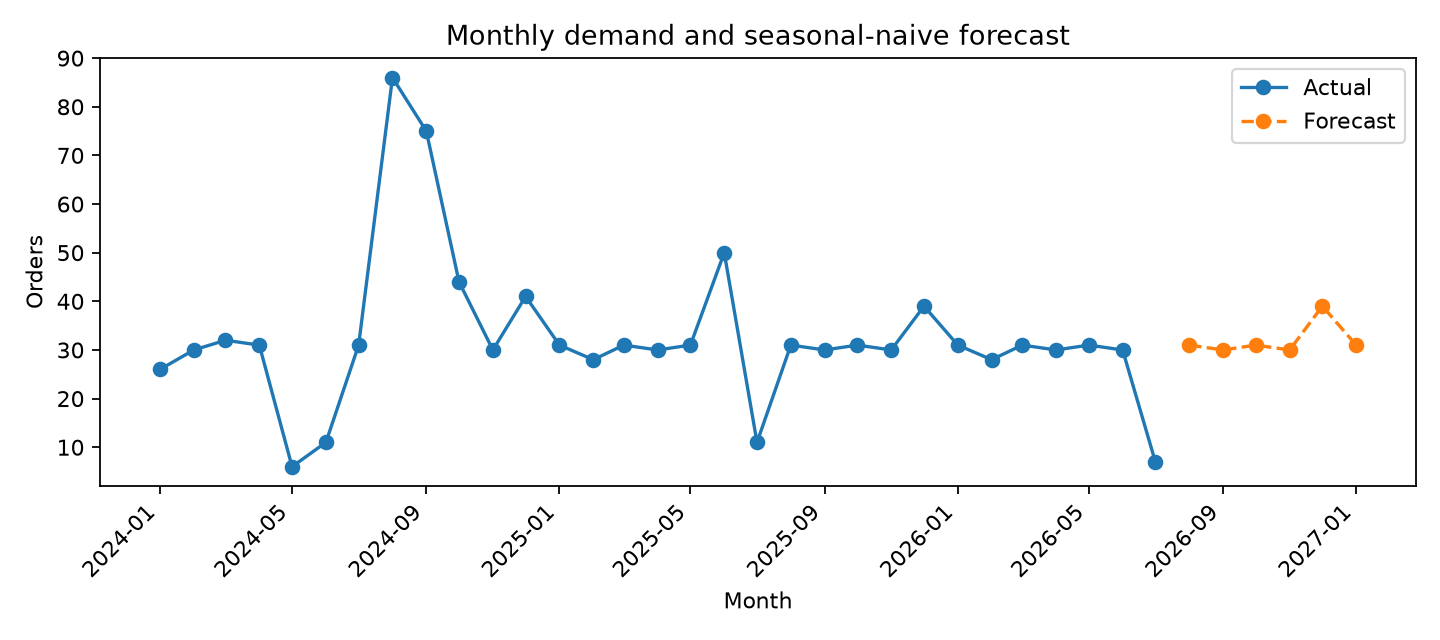
\includegraphics[width=\linewidth,height=0.6\textheight,keepaspectratio]{monthly_demand_forecast.png}
        \readfig{Đường dự báo (cam) bám trễ theo thực tế (xanh).}
    \end{columns}
\end{frame}

\begin{frame}{25. \mr Xếp ca theo giờ \& xu hướng sở thích}
    \begin{columns}[T]
        \column{0.5\linewidth}
        \blk{Xếp ca theo giờ}
        \begin{itemize}
            \item Cao điểm rơi vào \textbf{19h} hằng ngày.
            \item Đề xuất tăng nhân lực bếp giờ cao điểm thay vì rải đều.
        \end{itemize}
        \vspace{0.12cm}
        \blk{Xu hướng cỡ/loại bánh}
        \begin{itemize}
            \item Dự báo tỷ trọng đặt hàng từng cỡ/loại trong các tháng tới.
            \item Có vài xu hướng ``có ý nghĩa'', nhưng do dữ liệu giả lập nên phải coi là \textbf{đặc tính của bộ sinh dữ liệu}, không phải thị hiếu thật.
        \end{itemize}

        \column{0.48\linewidth}
        \centering
        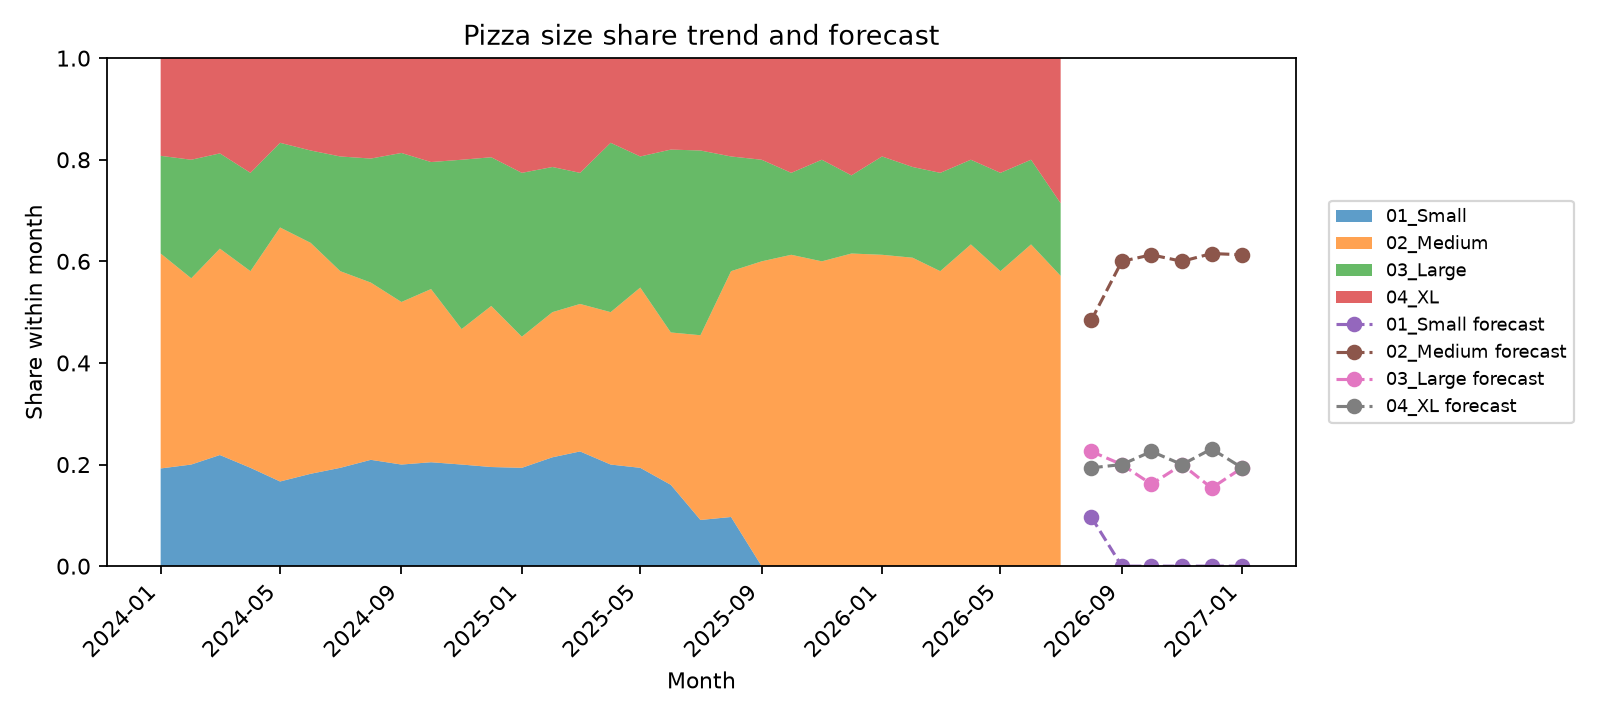
\includegraphics[width=\linewidth,height=0.6\textheight,keepaspectratio]{preference_size_share_forecast.png}
        \readfig{Tỷ trọng các cỡ bánh theo tháng + đoạn dự báo.}
    \end{columns}
\end{frame}

\begin{frame}{26. Đối chiếu rubric chấm điểm môn học}
    \begin{center}\small Bốn nhóm yêu cầu của phiếu chấm — dự án phủ ở các phần sau:\end{center}
    \vspace{-2pt}
    \begin{table}
        \centering
        \footnotesize
        \renewcommand{\arraystretch}{1.2}
        \begin{tabular}{p{3.7cm}p{6.6cm}p{1.9cm}}
        \toprule
        \textbf{Nhóm yêu cầu} & \textbf{Dự án thể hiện} & \textbf{Trạng thái}\\
        \midrule
        1. Xử lý dữ liệu (2đ) & Bài toán, tiền xử lý, thống kê, xử lý mất cân bằng & \textbf{\color{hustprimary}Đủ}\\
        2. Đánh giá mô hình (1đ) & Tiêu chí F2/MCC, 2 baseline, phân tích lỗi & \textbf{\color{hustprimary}Đủ}\\
        3. Cải tiến mô hình (4đ) & 6 mô hình + tinh chỉnh + bảng mô tả chi tiết & \textbf{\color{hustprimary}Đủ}\\
        4. Đóng gói (3đ) & Ứng dụng, demo Streamlit, slide, thuyết trình & \textbf{\color{hustprimary}Đủ}\\
        \quad (mô hình deep mới + paper) & Nêu rõ ở phần Giới hạn (dữ liệu bảng nhỏ) & Một phần\\
        \bottomrule
        \end{tabular}
    \end{table}
    \vspace{2pt}
    \begin{center}\footnotesize\itshape Chi tiết đối chiếu 20 mục: xem Bảng 7.1 trong báo cáo.\end{center}
\end{frame}

\begin{frame}{27. Bảng điều khiển — tổng quan \& khám phá}
    \begin{columns}[T]
        \column{0.45\linewidth}
        \blk{Trang tổng quan}
        \begin{itemize}
            \item Theo dõi nhanh: số đơn, tỷ lệ trễ, số đơn rủi ro cao cần can thiệp.
        \end{itemize}
        \vspace{0.12cm}
        \blk{Trang khám phá dữ liệu}
        \begin{itemize}
            \item Lọc tỷ lệ trễ theo từng yếu tố (giao thông, cỡ bánh, cửa hàng).
            \item Bảng \& biểu đồ trực quan cho người điều phối.
        \end{itemize}

        \column{0.53\linewidth}
        \centering
        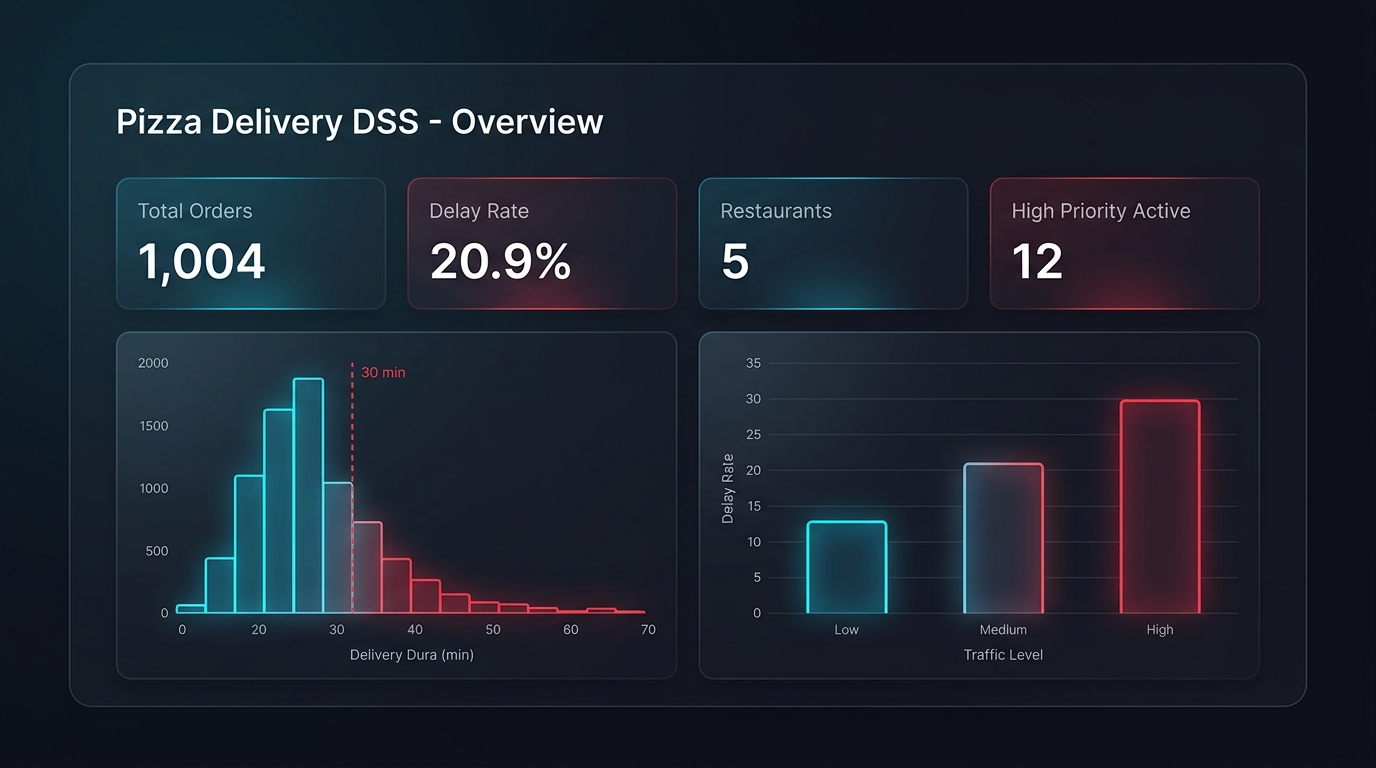
\includegraphics[width=\linewidth,height=0.66\textheight,keepaspectratio]{dashboard_overview.jpg}
    \end{columns}
\end{frame}

\begin{frame}{28. Bảng điều khiển — ra quyết định \& chất lượng dữ liệu}
    \begin{columns}[T]
        \column{0.45\linewidth}
        \blk{Trang thử một đơn}
        \begin{itemize}
            \item Nhập một đơn mới, hệ thống hiện điểm rủi ro \& \textbf{bóc tách} từng thành phần.
        \end{itemize}
        \vspace{0.1cm}
        \blk{Trang hàng đợi}
        \begin{itemize}
            \item Danh sách đơn ưu tiên kèm gợi ý xếp tài xế.
        \end{itemize}
        \vspace{0.1cm}
        \blk{Trang chất lượng dữ liệu}
        \begin{itemize}
            \item Hiện trực tiếp cảnh báo dữ liệu giả lập để kiểm duyệt.
        \end{itemize}

        \column{0.53\linewidth}
        \centering
        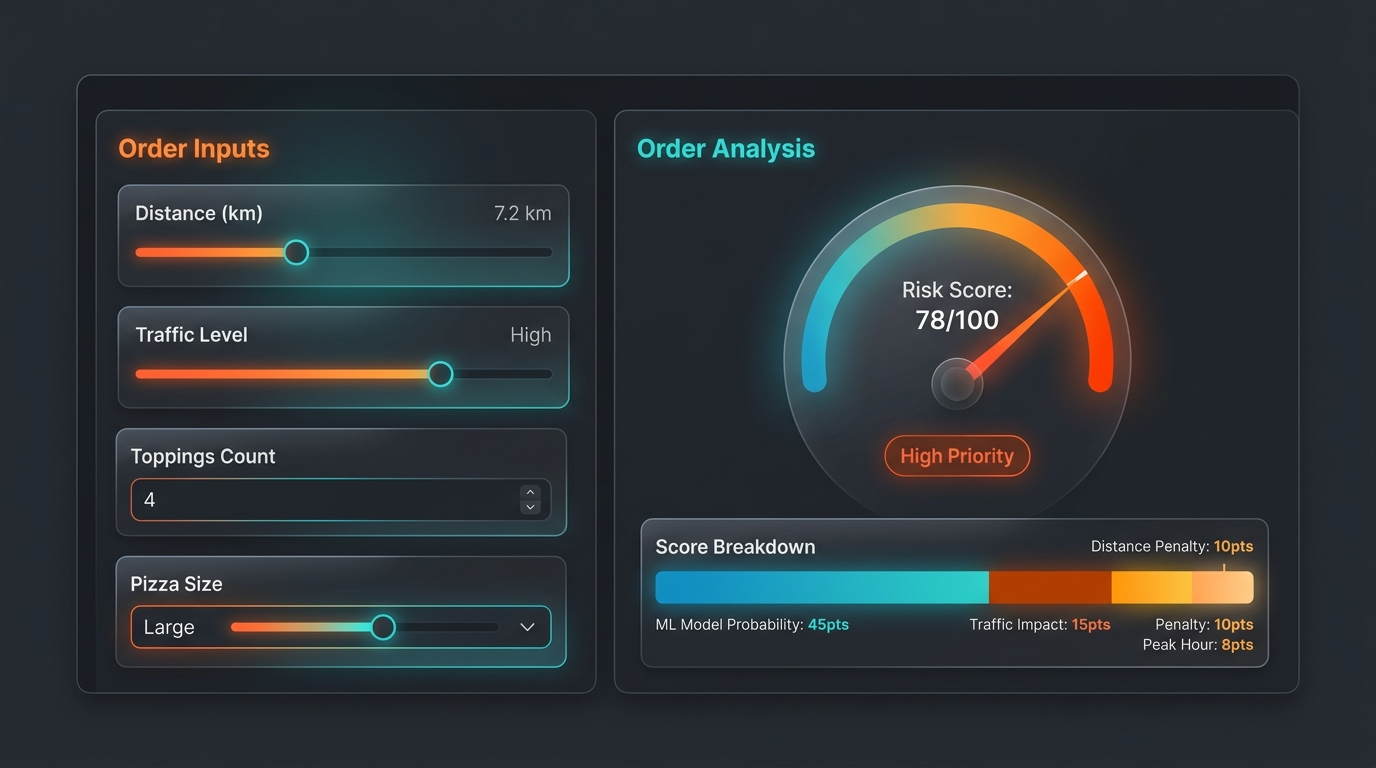
\includegraphics[width=\linewidth,height=0.66\textheight,keepaspectratio]{dashboard_single_order.jpg}
    \end{columns}
\end{frame}

\begin{frame}{29. Bộ dữ liệu báo cáo \& khả năng tái lập}
    \begin{columns}[T]
        \column{0.52\linewidth}
        \blk{Bộ dữ liệu cho Power BI}
        \begin{itemize}
            \item Các bảng dữ liệu sạch kèm công thức tính sẵn.
            \item Có hướng dẫn nạp dữ liệu \& dựng từng trang báo cáo.
        \end{itemize}
        \vspace{0.12cm}
        \blk{Tái lập hoàn toàn}
        \begin{itemize}
            \item Một lệnh dựng lại toàn bộ kết quả (chạy đủ 18 bước).
            \item Bộ kiểm thử tự động chạy đạt toàn bộ.
        \end{itemize}

        \column{0.46\linewidth}
        \blk{Các bước chạy}
        \begin{block}{}
        \scriptsize
        \texttt{python -m scripts.run\_all}\\
        \texttt{python -m unittest discover -s tests}\\
        \texttt{streamlit run app/streamlit\_app.py}
        \end{block}
        \footnotesize\itshape Mọi số liệu sinh ở một nơi; báo cáo và slide chỉ đọc
        lại để trình bày.
    \end{columns}
\end{frame}

\begin{frame}{30. Câu hỏi phản biện (1/2)}
    \begin{itemize}
        \item \textbf{Vì sao không dùng thời gian giao làm đặc trưng?}\\
              Đó là thông tin chỉ có sau khi giao; nó quyết định nhãn trễ nên dùng sẽ gây \textbf{rò rỉ} (điểm ảo).
        \vspace{0.3cm}
        \item \textbf{Ngưỡng trễ 30 phút ở đâu ra?}\\
              \textbf{Dò tự động} trên dữ liệu cho thấy khớp tuyệt đối tại mốc này, không phải nhóm tự đặt.
        \vspace{0.3cm}
        \item \textbf{Vì sao không chia tập theo thời gian?}\\
              20\% cuối theo thời gian \textbf{không có đơn trễ nào} nên không kiểm thử được; nhóm dùng cách chia giữ nguyên tỷ lệ lớp và ghi rõ giới hạn.
    \end{itemize}
\end{frame}

\begin{frame}{31. Câu hỏi phản biện (2/2)}
    \begin{itemize}
        \item \textbf{Điểm 96\% có nghĩa mô hình ``giỏi'' ngoài đời?}\\
              Không. Cao là vì dữ liệu gần như cố định (giả lập). Giá trị thật của đồ án là \textbf{quy trình \& truy vết}, không phải con số.
        \vspace{0.3cm}
        \item \textbf{Điểm rủi ro \& xếp tài xế có tối ưu thật?}\\
              Không. Điểm rủi ro là \textbf{chính sách trọng số minh bạch}; phần xếp tài xế dùng đội xe giả lập vì dữ liệu thiếu thông tin tài xế.
        \vspace{0.3cm}
        \item \textbf{Các phân tích mở rộng có tin được không?}\\
              Chỉ là \textbf{minh hoạ quy trình}. Mọi kết luận đều kèm ghi chú ``do bộ sinh dữ liệu'', không áp cho thị trường thật.
    \end{itemize}
\end{frame}

\begin{frame}{32. Giới hạn \& điều phải lưu ý}
    \begin{columns}[T]
        \column{0.48\linewidth}
        \blk{Giới hạn dữ liệu}
        \begin{itemize}
            \item Dữ liệu \textbf{giả lập}, cỡ nhỏ (1.004 dòng).
            \item Dự báo nhu cầu \& xu hướng chỉ minh hoạ cách làm.
            \item Không có vị trí tài xế thật, không có phản hồi khách thật.
        \end{itemize}

        \column{0.48\linewidth}
        \blk{Phải nói rõ khi trình bày}
        \begin{itemize}
            \item Không quảng cáo điểm 96\% là năng lực dự đoán thật.
            \item Không kết luận cửa hàng nào vận hành tốt hơn — chỉ là đặc tính bộ dữ liệu.
            \item Điểm rủi ro chưa tối ưu theo chi phí kinh doanh thật.
        \end{itemize}
    \end{columns}
\end{frame}

\begin{frame}{33. Kết luận \& hướng phát triển}
    \begin{columns}[T]
        \column{0.48\linewidth}
        \blk{Kết luận}
        \begin{itemize}
            \item Hoàn thành một hệ hỗ trợ quyết định \textbf{khép kín}: từ phân tích, dự đoán đến quyết định và xếp tài xế.
            \item Kiểm soát rò rỉ \& truy vết dữ liệu chặt chẽ.
            \item Chính sách quyết định minh bạch cho quản lý.
        \end{itemize}

        \column{0.48\linewidth}
        \blk{Hướng phát triển}
        \begin{itemize}
            \item Kết nối dữ liệu thật \& nhật ký vị trí tài xế.
            \item Tích hợp chi phí kinh doanh thật để tinh chỉnh điểm rủi ro.
            \item Tự động cập nhật trọng số theo phản hồi vận hành.
        \end{itemize}
    \end{columns}
\end{frame}

% =====================================================================
\hustthankyou

\end{document}
